\section{RESULTADO E DISCUSSÃO}
    % apresentação dos resultados obtidos, e discussão sobre os resultados obtidos

    \ipar Nesta seção serão apresentados os resultados obtidos com a implementação dos modelos de redes neurais e otimização de carteiras. Os resultados serão apresentados em duas etapas. A primeira etapa consiste na avaliação da otimização de carteiras, e a segunda etapa consiste na avaliação dos modelos de redes neurais.

    \subsection{OTIMIZAÇÃO COM PARÂMETROS REAIS}

        \ipar Em um primeiro momento, foi implementada a otimização de carteiras com base na equação \refeq{eq:sharpe}, modelo de Sharpe, utilizando o otimizador \acrshort{SLSQP} para o \acrshort{IBOVESPA}. A figura \ref{fig:otimizacao_ibov} apresenta a evolução do cálculo para obter a carteira ótima. No cálculo foi considerado a média e desvio padrão dos últimos 30 dias e risco igual a taxa SELIC para o último dia de junho de 2023.

        \begin{figure}[H]
            \centering
            \caption{Evolução da convergência de otimização da carteira}
            \label{fig:otimizacao_ibov}
            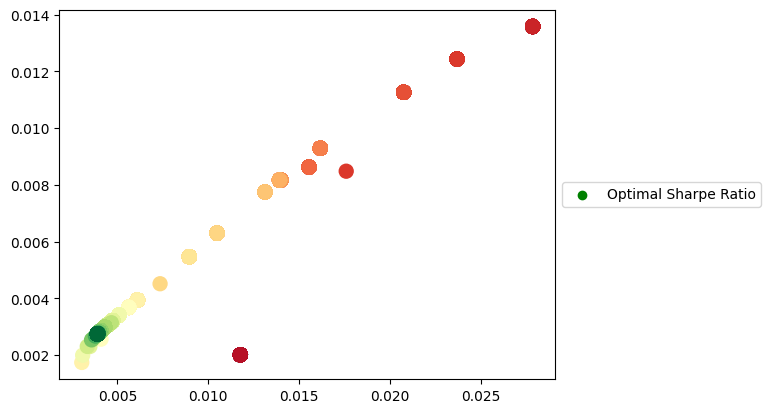
\includegraphics[width=0.5\textwidth]{./imagens/otimizacao_ibov.png}
            \par \footnotesize Fonte: próprio autor.
        \end{figure}

        \ipar Os pontos estão ordenados em escala de cor, do vermelho ao verde, e amarelo o intermediário. O otimizador converge para um ponto de máximo, o ponto verde, que representa a carteira de mercado de \citeonline{sharpe1964capital}. Contudo, este modelo contém somente a restrição de que a soma das porcentagens de alocação deve ser igual a um, o que na prática pode não ser possível. Os ativos financeiros são negociados em lotes, e não é possível comprar 0,5\% de uma ação, além disso, o capital de investimento é limitado. 

        \ipar Para avaliar a carteira ótima com parâmetros reais em comparação ao modelo de Sharpe sem restrições adicionais, foi realizada a otimização em três cenários. Os cenários são dados pela média e desvio padrão dos últimos 15, 30 e 60 dias nos componentes do \acrshort{IBOVESPA}. 

        \ipar O modelo com restrições reais foi implementado com o otimizador APOPT. O mo-delo matemático segue a equação \refeq{eq:otimizacao}. Este modelo considera capital de investimento, custos de operação, cotação e lotes de negociação, rebalanceamento, aversão ao risco e somente posições de compra. As restrições da equação contém parâmetros de mercado, como a cotação e lotes de negociação, e parâmetros de investimento, como o capital de investimento e custos de operação. Os dados destes parâmetros foram obtidos conforme descrito no quadro \ref{quadro:coleta_dados}. Os demais parâmetros foram definidos conforme o quadro \ref{quadro:parametros}.

        \begin{table}[H]
            \centering
            \caption{Parâmetros de mercado e investimento}
            \label{quadro:parametros}
            \begin{tabular}{ll}
                \hline
                \textbf{Parâmetro} & \textbf{Valor} \\
                \hline
                Capital de Investimento & R\$ 20.000,00 \\
                Valor Monetário Aceitável de Perda Diária & R\$ 100,00 \\
                Quantil da Distribuição Normal Padrão ao Nível de Confiança & 95\% \\
                Quantidade Inicial de Lotes do Ativo & 0 \\
                \hline
            \end{tabular}
            \par \footnotesize Fonte: próprio autor.
        \end{table}

        \ipar Com todos os parâmetros e dados definidos, foi realizada a otimização com otimizador APOPT. Como resultado, este otimizador não conseguiu realizar a tarefa devido à complexidade do problema, quando considerados os 87 componentes listados da \acrshort{IBOVESPA}. Após a avaliação da literatura, optou-se por utilizar a heurística de busca básica no núcleo de \citeonline{angelelli2012kernel}. Contudo, para este estudo, optou-se pela aplicação das duas primeiras etapas do algoritmo. A primeira etapa consiste em uma busca aleatória, e a segunda etapa consiste em uma busca local. 

        \ipar Por se tratar de um problema não linear com variáveis discretas, o algoritmo está suscetível a mínimos locais, com dependência da posição inicial. Para contornar este problema, foi implementada à uma distribuição aleatória, a distribuição de Dirichlet. Portanto, neste estudo serão comparado os resultados e tempo computacional da otimização com e sem a heurística de busca básica, e com e sem restrições reais para os três cenários. A tabela \ref{tab:resultados_opt} apresenta os resultados obtidos.

        \begin{table}[htbp]
            \centering
            \caption{Resultados da otimização para os três cenários}
            \label{tab:resultados_opt}
            \resizebox{\columnwidth}{!}{%
            \begin{tabular}{clrrrr}
                \hline
                \textbf{Carteira} & \textbf{Método} & \textbf{Retorno} & \textbf{Risco} & \textbf{Sharpe do Otimizador} & \textbf{Tempo (s)} \\ \hline \hline
                15 & Sem Restrições & 15.80 & 16.14 & 0.9791 & 0.42 \\
                15 & Restrições e Aleatório & 3.96 & 39.83 & -0.0849 & 3.81 \\
                15 & Restrições com Heurística & 10.90 & 14.99 & 0.0751 & 3.70 \\
                30 & Sem Restrições & 43.98 & 61.49 & 0.7152 & 0.20 \\
                30 & Restrições e Aleatório & 23.37 & 121.18 & 0.1191 & 3.92 \\
                30 & Restrições com Heurística & 22.80 & 48.41 & 0.2321 & 3.88 \\
                60 & Sem Restrições & 64.01 & 106.91 & 0.5987 & 0.18 \\
                60 & Restrições e Aleatório & 1.15 & 48.36 & -0.1146 & 3.21 \\
                60 & Restrições com Heurística & 15.99 & 66.19 & -0.1700 & 10.13 \\
                \hline
            \end{tabular}%
            }
            \par \footnotesize Fonte: próprio autor.
        \end{table}

        \ipar Para a comparação dos resultados, os valores de porcentagem do modelo sem restrições foi multiplicado pelo capital disponível. As colunas de risco e retorno da tabela \ref{tab:resultados_opt} estão em valores monetários, em real. A coluna de Sharpe do otimizador é o valor obtido pelo processo de otimização, enquanto os valores de retorno e risco foram calculados após o processo dada a quantidade de lotes do ativo, pela cotação, a média e risco por cada ativo antes de os custos serem aplicados. Assim, os valores de Sharpe negativos são devido à consideração do custo de operação durante o cálculo. 

        \ipar Avaliando o índice Sharpe, é possível observar que o modelo sem restrições supera significativamente os outros modelos, além do tempo de otimização ser inferior. Enquanto o modelo sem restrições dura no máximo 0,42 segundos, o modelo com restrições dura no mínimo 3,21 segundos. Para observar o efeito dos modelos na distribuição normal das carteiras, foi feito o gráfico de densidade de probabilidade das carteiras, apresentado na figura \ref{fig:densidade_carteiras}.

        \begin{figure}[H]
            \centering
            \caption{Densidade de probabilidade das carteiras.}
            \label{fig:densidade_carteiras}
            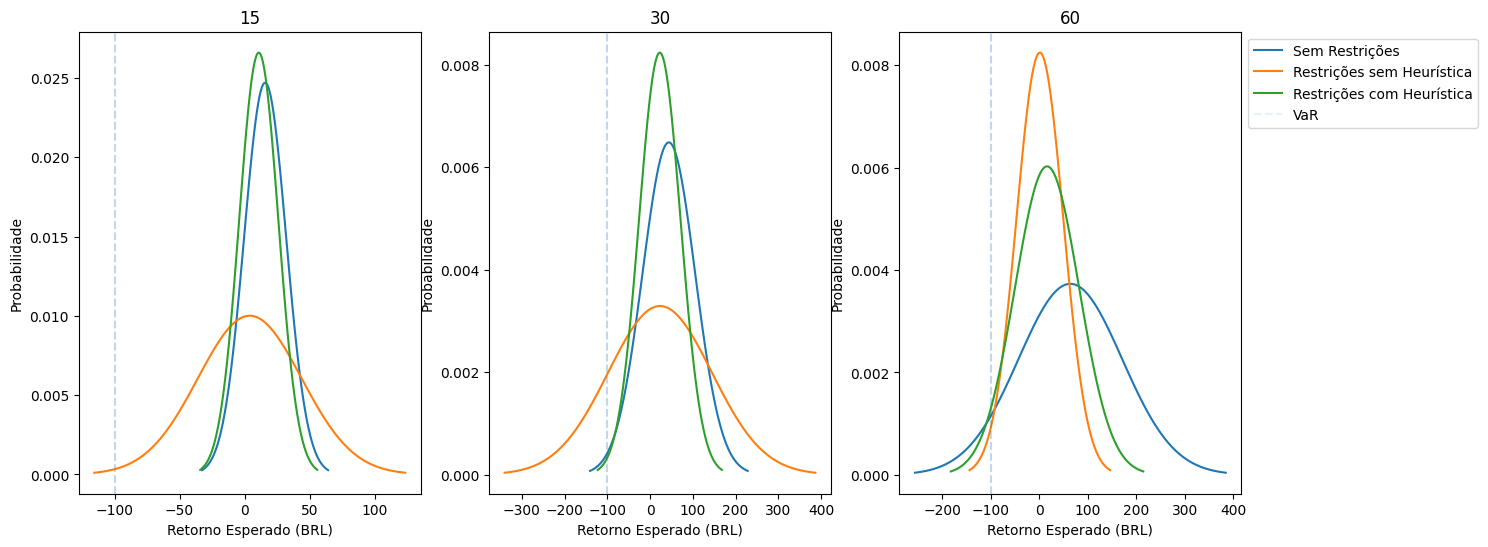
\includegraphics[width=\textwidth]{./imagens/distribuicao_carteiras.png}
            \par \footnotesize Fonte: próprio autor.
        \end{figure}

        \ipar A linha vertical na figura \ref{fig:densidade_carteiras} representa o limite aceitável de perda para o investidor. A carteira com início aleatório não conseguiu atender esta restrição. Este efeito não foi possível de identificar na referência do modelo \cite{hedengren2014nonlinear}. As demais carteiras atendem a restrição. Há um efeito de estreitamento da distribuição da carteira com restrições e heurística, em relação à carteira sem restrições, e um deslocamento negativo do retorno. Isso ocorre devido à inclusão dos custos de operação e a restrição de perda máxima.

        \ipar A tabela \ref{tab:distribuicao_carteira_30} apresenta alocação da carteira de 30 dias para os modelos sem restrição e com restrição e heurística. 

        \begin{table}[htbp]
            \centering
            \caption{Alocação da carteira de 30 dias}
            \label{tab:distribuicao_carteira_30}
            \begin{tabular}{rrr}
                \hline
                & Sem Restrições & Restrições com Heurística \\
                \hline\hline
               BRKM5 & 480 & - \\
               ENBR3 & 15620 & 18912 \\
               EQTL3 & 1400 & - \\
               GOLL4 & 80 & - \\
               IRBR3 & 820 & - \\
               JBSS3 & 520 & - \\
               PRIO3 & 540 & - \\
               RAIZ4 & 480 & - \\
               SLCE3 & 40 & - \\
               Livre de Risco & - & 1088 \\
               \hline
            \end{tabular}
            \par \footnotesize Fonte: próprio autor. 
        \end{table}

        \ipar A carteira sem restrições apresenta uma alocação mais diversificada, enquanto a carteira com restrições e heurística apresenta uma alocação mais concentrada. A carteira com restrições e heurística apresenta uma alocação de 1088 reais em ativos de baixo risco, enquanto a carteira sem restrições não apresenta alocação em ativos de baixo risco. A alocação em ativos de baixo risco é devido à restrição de perda máxima. A carteira sem restrições apresenta uma alocação de 15620 reais em ENBR3, enquanto a carteira com restrições e heurística concentra o investimento neste ativo. Isto ocorre devido ao método heurístico utilizar o resultado do modelo sem restrições como o conjunto de ativos candidatos para a seleção da carteira. E como muitos dos ativos tem valor inferiores ao tamanho mínimo de compra por lote, o modelo com restrições e heurística não consegue selecionar estes ativos.

        \ipar Portanto, é possível concluir que o modelo sem restrições apresenta um melhor desempenho, em relação ao tempo de otimização e ao índice Sharpe. O modelo com restrições e heurística apresenta um desempenho inferior, porém atende a restrição de perda máxima, com exceção do modelo com início aleatório.
        

    \subsection{REDES NEURAIS}
        % apresentação dos resultados obtidos, e discussão sobre os resultados obtidos
    
        \ipar A aplicação das redes neurais, visa a seleção da carteira de melhor desempenho no próximo período. Foi realizado a otimização de 3 carteiras dinâmicas de investimentos, isto é com atualização regular dos ativos. As carteiras são de 15, 30 e 60 dias de intervalo para média e desvio padrão. Após a otimização das carteiras com atualização diária, é feito a comparação dos retornos gerados pelas carteiras selecionadas no período de análise. A figura \ref{fig:boxplot_inv} apresenta os retornos gerados pelas carteiras.

        \begin{figure}[H]
            \centering
            \caption{Retornos gerados pelas carteiras.}
            \label{fig:boxplot_inv}
            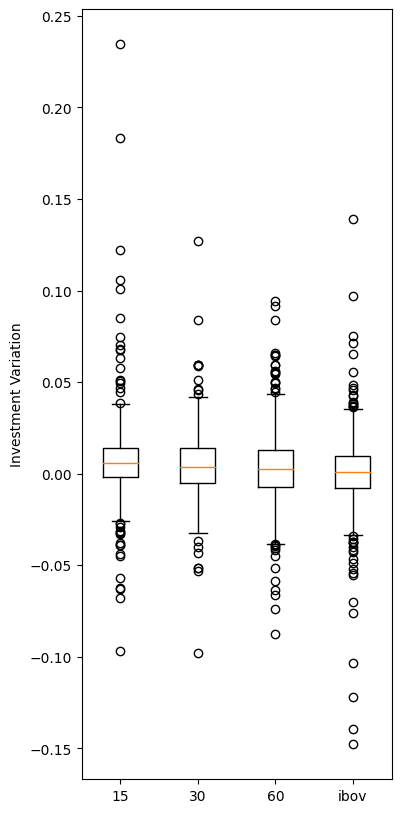
\includegraphics[width=0.25\textwidth]{./imagens/boxplot_inv.png}
            \par \footnotesize Fonte: próprio autor.
        \end{figure}

        \ipar Pela figura \ref{fig:boxplot_inv}, nota-se que a carteira de referência, \acrshort{IBOVESPA} e a de 15 dias apresentam as maiores dispersões de retorno, enquanto as carteiras de 30 e 60 dias apresentam menor dispersão. Dentre as carteiras, não é possível observar uma carteira com retorno significativamente superior. Plotando o retorno acumulado das carteiras para os últimos 120 dias do período de análise é possível observar a evolução dos retornos, conforme a figura \ref{fig:retorno_acumulado}.

        \begin{figure}[H]
            \centering
            \caption{Retorno acumulado das carteiras.}
            \label{fig:retorno_acumulado}
            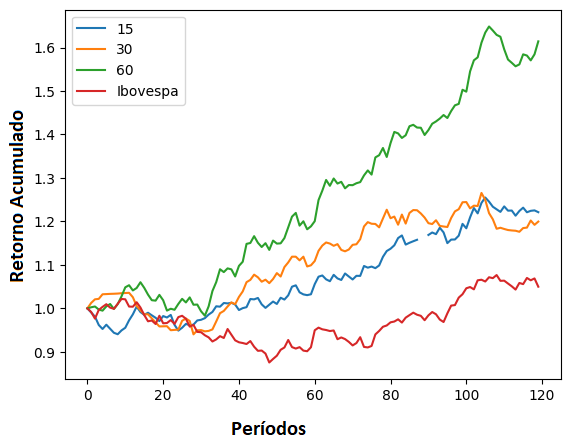
\includegraphics[width=0.6\textwidth]{./imagens/retorno_acumulado.png}
            \par \footnotesize Fonte: próprio autor.
        \end{figure}

        \ipar Pela figura \ref{fig:retorno_acumulado} é possível observar que a carteira de 60 dias apresenta o maior retorno acumulado. Nota-se que as carterias em geral apresentaram retornos superiores ao \acrshort{IBOVESPA}. Além disso, é possível observar que a carteira de 15 dias apresenta intervalos faltantes, isso ocorre devido à falta de sucesso no processo de otimização. A figura \ref{fig:success_results} apresenta a porcentagem de sucesso na otimização das carteiras.

        \begin{figure}[H]
            \centering
            \caption{Porcentagem de sucesso na otimização das carteiras.}
            \label{fig:success_results}
            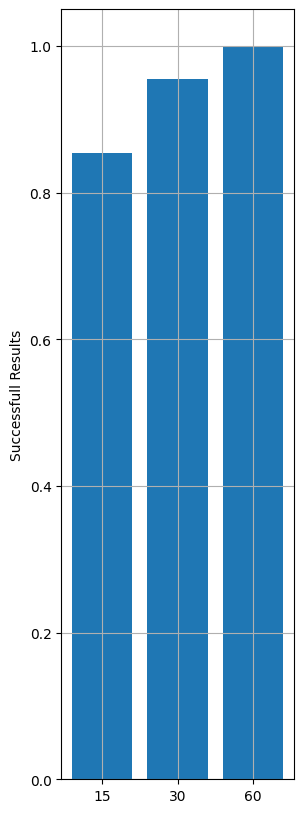
\includegraphics[width=0.15\textwidth]{./imagens/success_results.png}
            \par \footnotesize Fonte: próprio autor.
        \end{figure}

        \ipar A carteira de 15 dias, obteve mais de 10\% de falha na otimização, e a carteira de 30 dias menos de 5\% de falha. A de 60 dias não apresentou falha na otimização. Após avaliação, foi identificado a falha durante o processo de busca direcional durante a otimização por meio do método \acrshort{SLSQP}. Apesar disso, optou-se por manter os resultados, pois quando avaliado o alvo para rede neural, esta carteira não é definida como a melhor opção para o próximo período. 

        \ipar Para a aplicação da rede neural, foram propostas 4 estruturas de redes: \acrshort{LSTM}+Atenção de Bahdanau, \acrshort{LSTM}+Auto Atenção, \acrshort{GRU}+Atenção de Bahdanau, e \acrshort{GRU}+Auto Atenção. As estruturas das redes \acrshort{LSTM} são apresentadas nas figuras \ref{fig:model_lstm_BauhAtt} e \ref{fig:model_lstm_SelfAtt}, no qual são equivalentes para as redes \acrshort{GRU}. A rede neural foi treinada com 90\% dos dados e testada com 10\% dos dados, gerando 1198 dados para treino e 120 para teste. No treino foi realizado a validação cruzada com lacunas, considerando 10 partições, sendo 1 para teste, 6 para treino e duas parcelas anterior e uma após o teste não são consideradas. Para o treino dos hiperparâmetros, foi utilizada uma das parcelas da validação cruzada. A figura \ref{fig:loss} apresenta a função de perda para o treinamento de hiperparâmetros para a rede \acrshort{LSTM}+Atenção de Bahdanau.

        \begin{figure}[H]
            \centering
            \caption{Função de perda para o treinamento de hiperparâmetros.}
            \label{fig:loss}
            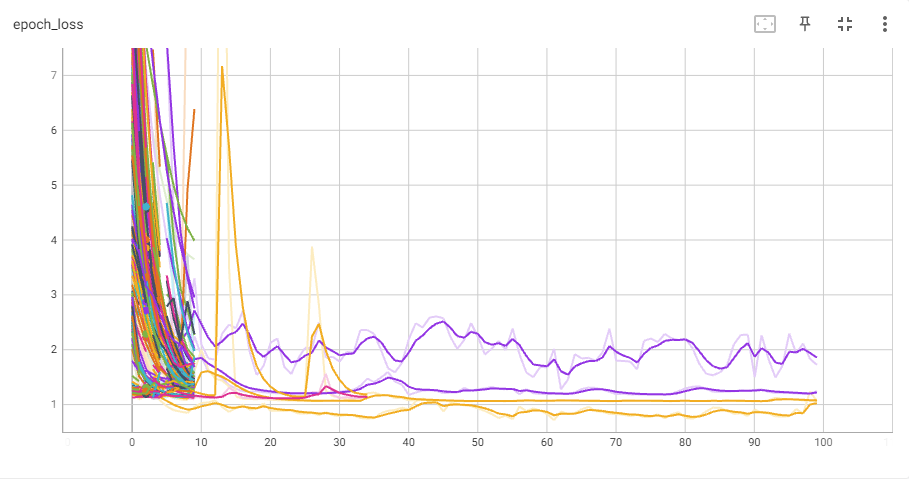
\includegraphics[width=0.8\textwidth]{./imagens/epoch_loss.png}
            \par \footnotesize Fonte: próprio autor.
        \end{figure}

        \ipar Pela figura \ref{fig:loss}, nota-se que a função de perda apresenta uma tendência de convergência, a qual é esperada para o treinamento de hiperparâmetros. A figura \ref{fig:loss} apresenta a função de perda para o treinamento da rede neural.

        \ipar Todas as demais redes passaram pelo processo de seleção de hiperparâmetros, e segui-ram para a avaliação pela validação cruzada. Após o treinamento da redes por este processo, é avaliada a acurácia, que é a proporção de acertos do modelo. A figura \ref{fig:accuracy} apresenta a acurácia para as redes avaliadas.

        \begin{figure}[H]
            \centering
            \caption{Acurácia para as redes avaliadas.}
            \label{fig:accuracy}
            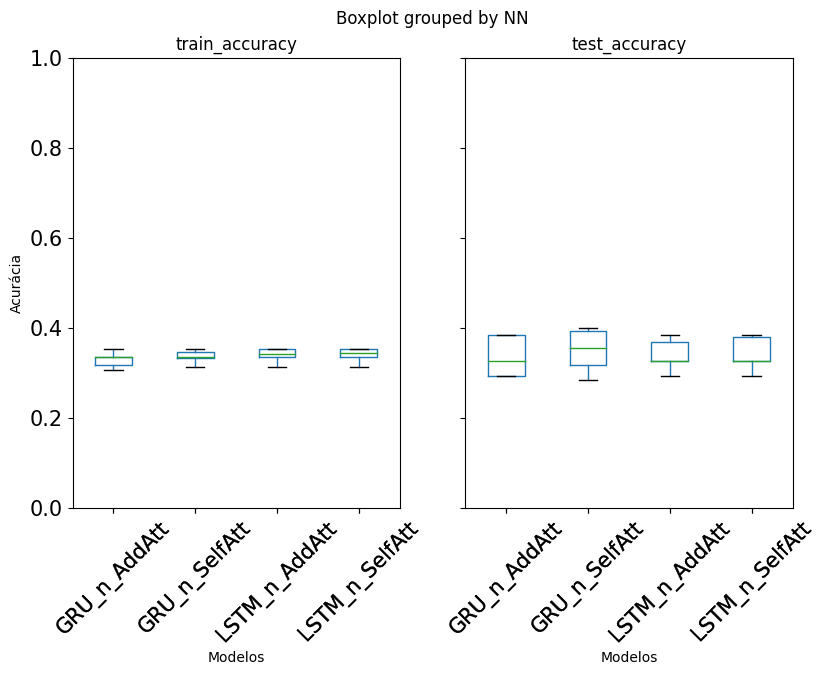
\includegraphics[width=0.7\textwidth]{./imagens/boxplot_val_01.png}
            \par \footnotesize Fonte: próprio autor.
        \end{figure}

        \ipar As redes apresentaram acurácia inferior a 40\%, o que indica que o modelo não é capaz de prever o retorno da carteira com precisão. A figura \ref{fig:boxplotval_zoom} apresenta uma visão ampliada da acurácia para as redes avaliadas.

        \begin{figure}[H]
            \centering
            \caption{Acurácia para as redes avaliadas ampliado.}
            \label{fig:boxplotval_zoom}
            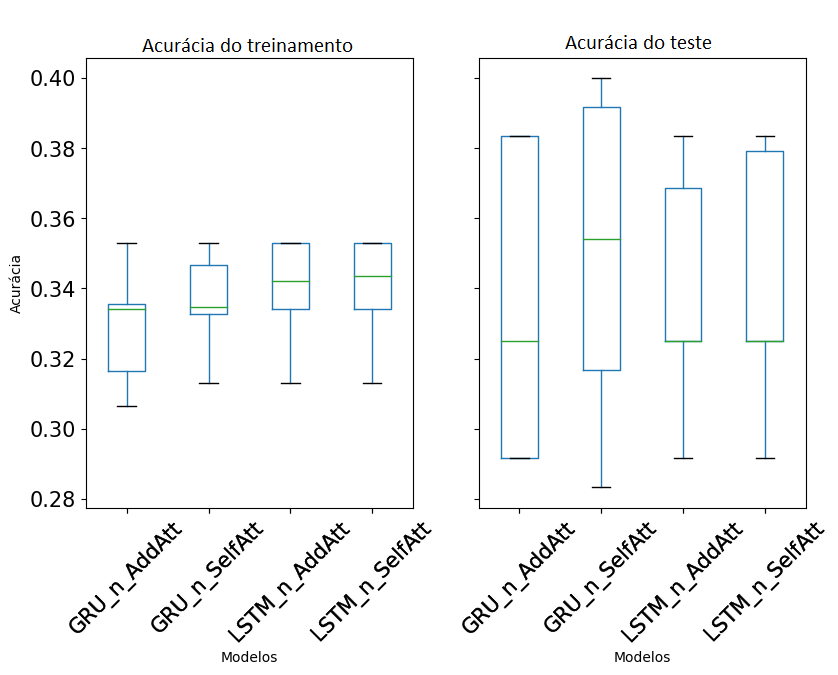
\includegraphics[width=0.7\textwidth]{./imagens/boxplotval_zoom.png}
            \par \footnotesize Fonte: próprio autor.
        \end{figure}

        \ipar A rede \acrshort{GRU}+Atenção de Bahdanau apresentou a menor acurácia, representada por 'GRU\_n\_AddAtt'. As demais redes apresentaram acurácia semelhante. Todas as redes apresentam uma acurácia próximo a 33\%,. A figura \ref{fig:freq} apresenta a frequência dos atributos alvos do teste para avaliar esta distribuição das carteiras a serem escolhidas.

        \begin{figure}[H]
            \centering
            \caption{Frequência dos atributos alvos do teste.}
            \label{fig:freq}
            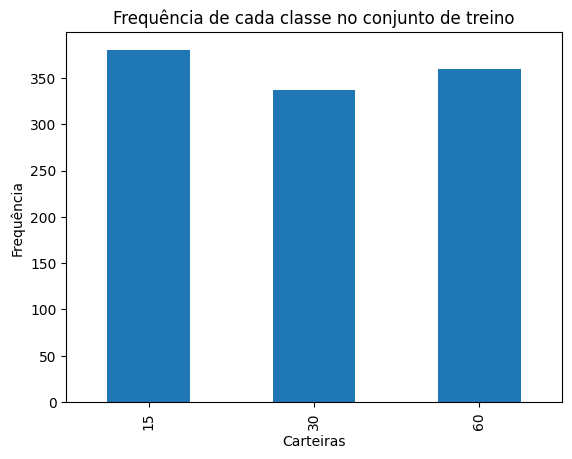
\includegraphics[width=0.5\textwidth]{./imagens/freq.png}
            \par \footnotesize Fonte: próprio autor.
        \end{figure}

        \ipar Portanto, as carteiras a serem escolhidas apresentam uma distribuição semelhante, o que indica que a acurácia obtida das redes são semelhantes a uma escolha de somente uma carteira, sendo esta feita de forma aleatória.

        \ipar Contudo, seguindo para a validação da capacidade de predição da rede neural, foram avaliadas as escolhas feitas pelas redes ao longo do tempo. Avaliando o período de teste, a figura \ref{fig:backtest_ts} apresenta a comparação das séries temporais geradas pelas predições das redes neurais, em comparação com as carteiras e o \acrshort{IBOVESPA}.

        \begin{figure}[H]
            \centering
            \caption{Séries temporais de retorno acumulado geradas pelas predições das redes neurais.}
            \label{fig:backtest_ts}
            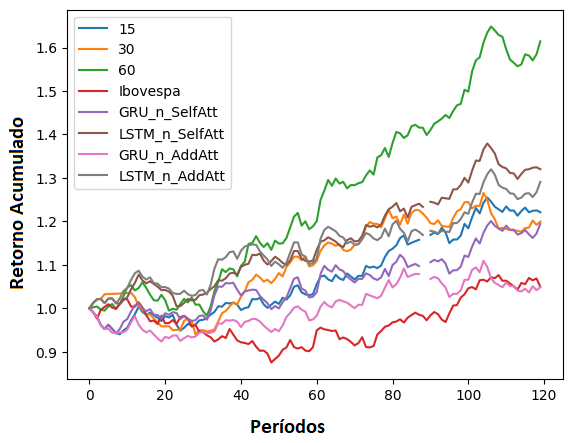
\includegraphics[width=0.6\textwidth]{./imagens/backtest_ts.png}
            \par \footnotesize Fonte: próprio autor.
        \end{figure}

        \ipar As redes neurais com \acrshort{GRU}, demonstraram resultados inferiores às próprias carteiras. A rede neural \acrshort{GRU}+Atenção de Bahdanau apresentou o pior resultado e, em alguns períodos, se manteve inferior ao \acrshort{IBOVESPA}. As redes neurais com \acrshort{LSTM} obtiveram os melhores resultados no retorno acumulado, contudo ainda inferior à carteira de melhor desempenho, a carteira de 60 dias. Os resultados diferem da literatura, em que \citeonline{cao2020delafo} encontra resultados superiores para a rede \acrshort{GRU}+Atenção de Bahdanau. Este estudo difere de \citeonline{cao2020delafo} na aplicação de atributos de entrada, em seu estudo é inserida a combinação de volume e preços de ativos, enquanto este estudo utiliza somente os preços de ativos. \citeonline{daiya2021stock}, que aplica a combinação de atenção com redes neurais convolucionais, também apresenta resultados superiores em seu estudo, contudo, os atributos de entrada são dados de análises técnicas de ativos. Portanto, a diferença de resultados pode ser atribuída aos atributos de entrada utilizados, sendo necessário um estudo mais aprofundado para avaliar a influência destes atributos.

        \ipar Com objetivo de avaliar o desempenho das redes quanto ao índice Sharpe, a tabela \ref{tab:sharpe} apresenta um comparativo entre as redes avaliadas e as carteiras. A tabela \ref{tab:sharpe} apresenta a média, desvio padrão e índice Sharpe em valores absolutos diários para as redes avaliadas e as carteiras.

        \begin{table}[htbp]
            \centering
            \caption{Índice Sharpe para as redes avaliadas e as carteiras.}
            \label{tab:sharpe}
            \begin{tabular}{rrrr}
                \hline
                & \textbf{Média} & \textbf{Desvio Padrão} & \textbf{Índice Sharpe} \\ \hline \hline
                GRU\_n\_SelfAtt & 0.0016 & 0.0119 & 0.13 \\
                LSTM\_n\_SelfAtt & 0.0024 & 0.0095 & 0.25 \\
                GRU\_n\_AddAtt & 0.0005 & 0.0105 & 0.04 \\
                LSTM\_n\_AddAtt & 0.0022 & 0.0114 & 0.19 \\
                15 & 0.0017 & 0.0101 & 0.17 \\
                30 & 0.0016 & 0.0108 & 0.15 \\
                60 & 0.0041 & 0.0131 & 0.31 \\
                \hline
                \par \footnotesize Fonte: próprio autor.
            \end{tabular}
        \end{table}

        \ipar A rede neural \acrshort{LSTM}+Atenção de Bahdanau apresentou o melhor índice Sharpe, seguido pela carteira de 60 dias. O que confirma o desempenho apresentado pela figura \ref{fig:backtest_ts}. 
 
\pagebreak